\subsection[Navigation mit dem Mikrofon]{Navigation mit dem Mikrofon \footnote{Diana Castano}}
\thispagestyle{fancy}

\subsubsection{Anforderungen}
Die Applikation setzte eine Navigation durch die PDF-Datei mithilfe des Mikrofons voraus, wodurch ein Klatschen oder Klopfen erkannt und als Blättern interpretiert werden konnte. Bei einmaligem oder zweimaligem Klatschen wurden entsprechende Signale zum vor- bzw. zurückblättern gesendet. \\
\\
Eine der Herausforderung dabei war, die Erkennung unabhängig von den äußeren Gegebenheiten erfolgen zu lassen (Raum mit oder ohne Nachhall). Außerdem sollte kein Signal zum Weiterschalten der Folien erzeugt werden, wenn ein starker Klang oder Ton aufgenommen wurde (z.B. wenn der Präsentator ggf. lauter sprechen musste). Der Algorithmus und die dabei berechneten Parameter sollten dabei nicht für jedes Gerät angepasst werden, selbst wenn die Mikrofone über unterschiedliche Eigenschaften verfügten. 

\subsubsection{Umsetzung}
Als erste Implementierung wurde eine Erkennung im Zeitbereich gewählt. Es wurde schnell festgestellt, dass dies eine sehr leise Umgebung voraussetzte. Selbst der Sprecher konnte das Signal aktivieren, wenn er sehr nah am Mikrofon war. Aus diesem Grund erfolgte die Erkennung im Frequenzbereich. Die Signalverarbeitung war hierbei aufwändiger, allerdings wurden damit die Herausforderungen überwunden.\\
\\
Das Modul  \href{http://doc.qt.io/qt-5/qtmultimedia-index.html}{Qt Multimedia 5.7} stellt verschiedene C++ Klassen zur Verfügung, die für die Steuerung des Mikrofons hilfreich sind. Eine Abfrage über die verfügbaren Aufnahmegeräte konnte mit \textit{QAudioDeviceInfo} durchgeführt werden. Das Audio-Format und die Darstellung der Daten wurden mithilfe der Klasse \textit{QAudioFormat} festgelegt. Folgende Einstellungen wurden verwendet:

\begin{center}
	\begin{itemize}
		\item Abtastrate: 8 kHz
		\item Anzahl der Kanäle: 1 (mono)
		\item Bytes pro Abtastwert: 2
		\item Format der Abtastwerte: Signed Integer
		\item Byte-Reihenfolge: Little Endian
		\item Codec: Linear PCM	
	\end{itemize}
\end{center}

Die Klasse \textit{QAudioInput} bietet eine Schnittstelle um akustische Signale aus einem Mikrofon aufzunehmen. Dafür muss zuerst ein Aufnahmegerät mithilfe von \textit{QIODevice} im Lesemodus zum Empfangen der Daten geöffnet werden. Jede Sekunde werden neue Daten aus dem Mikrofon gelesen. Die Daten, die sich im Buffer befindet werden zuerst in einem \textit{QByteArray} gespeichert. Anschließend werden die Abtastwerte vom \textit{Signed Integer} Format zum \textit{Float} umgewandelt und in einem \textit{QVector} gespeichert, um eine Fourier-Analyse des Signals zu ermöglichen.\\
\\
Die Analyse im Frequenzbereich erfolgt durch das Spektrogramm, das eine Zusammensetzung des akustischen Signals in seinen einzelnen Frequenzen im zeitlichen Verlauf darstellt. Dafür müssen zuerst die im Buffer gespeicherten Abtastwerte in sich überlappende Rahmen aufgeteilt werden, wie in \autoref{fig:image0} dargestellt wird:

\begin{figure}[h]
	\centering
	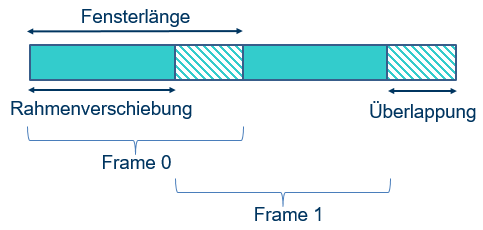
\includegraphics[width=1\textwidth]{beatcontrol/BeatBilder/bild0.png}
	\caption{Aufteilung des Signals in Rahmen}
	\label{fig:image0}
\end{figure}

Dafür wurden folgende Größen gewählt:
 
\begin{center}
	\begin{itemize}
		\item Länge des Buffers: 16000 Bytes
		\item Länge der einzelnen Rahmen: 256 Werte (circa 25 ms)
		\item Rahmenverschiebung: 80 Werte (10 ms)
		\item Überlappung: 176 Werte
		\item Anzahl von Rahmen: 98
		\item Fenstertyp: Hanning
	\end{itemize}
\end{center}


Falls das Signal sich nicht in genau dieser Anzahl von Rahmen aufteilen lässt, werden Nullen am Ende des Signals hinzugefügt. Da die Länge der Rahmen endlich ist und kein Vielfaches der Periode des Signals darstellt, müssen die Rahmen mit einer Fensterfunktion gewichtet werden, um den Leck-Effekt zu vermeiden.  \\
\\
Anschließend muss die Diskrete Fourier-Transformation (DFT) für jeden Rahmen berechnet werden. Die Schnelle-Fourier Transformation (FFT) ist ein effektiver Algorithmus zur Berechnung der DFT. Für die Implementierung der FFT in Qt 5.7 wurde die Open-Source Bibliothek \href{ http://ldesoras.free.fr/prod.html}{FFTReal} verwendet, die für schnelle Berechnungen optimiert ist (besonders wenn die Anzahl der FFT-Punkte schon bekannt ist). \\
\\
Es wurde zunächst der Betrag der Transformation berechnet, daraufhin erfolgte die Berechnung des Logarithmus. Folge dessen wurden die Ergebnisse in Form einer Matrix in einer CSV-Datei gespeichert. Die Spalten stellen die einzelnen Rahmen dar (Zeitindex), wobei die Reihen der Frequenzanteile (Frequenzindex) entsprechen. Anschließend wurde die Datei mit MATLAB gelesen und geplottet. \autoref{fig:image1} zeigt eine farbcodierte Darstellung dieser Matrix: \\

\begin{figure}[h]
	\centering
	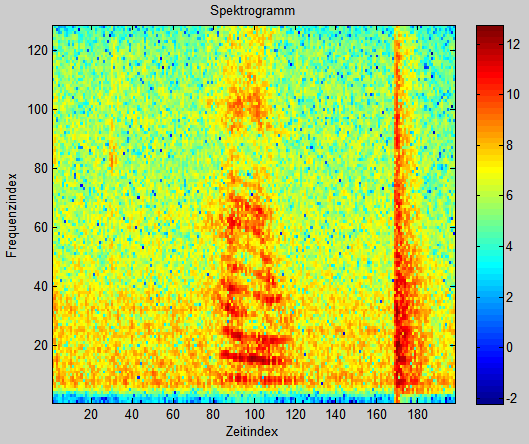
\includegraphics[angle=0,width=14cm]{beatcontrol/BeatBilder/bild1.png}
	\caption{Spektrogramm ("`Hallo"' $+$ Klatschen)}
	\label{fig:image1}
\end{figure}

Hier ist die zeitliche Entwicklung aller Frequenzkomponenten des Signals zu sehen. In diesem Fall wurde ein "`Hallo"' und folglich ein Klatschen aufgenommen. Dabei wird deutlich, dass ein Klatschen ein sehr breitbandiges Signal erzeugt, in welchem alle Frequenzen erhalten sind. Ein "`Hallo"' hingegen enthält nur bestimmte und wenige Frequenzanteile. Es wurde festgestellt, dass die Erkennung auf dieser Analyse erfolgen konnte. \\
\\
Der Algorithmus berechnet die Summe der Frequenzanteile jeder Rahmen, wie in \autoref{fig:image2} zu sehen ist (in diesem Fall wurden zwei Klatschen aufgenommen). Wenn die Summe eine bestimmte Schwelle überschreitet, und der darauffolgende Wert wiederum kleiner ist, wird dies als ein Klatschen erkannt. Anschließend wird für eine Sekunde ein Timer gestartet. Wenn innerhalb dieser Zeit die gleiche Erkennung erfolgt, wird das Signal zum Zurückblättern gesendet. Ansonsten wird das Signal zum Vorblättern gesendet.

\begin{figure}[H]
	\centering
	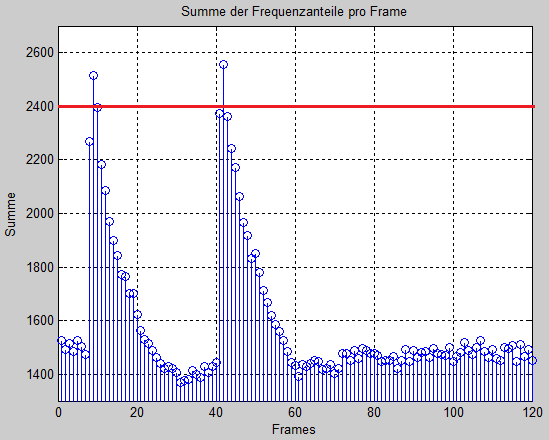
\includegraphics[angle=0,width=14cm]{beatcontrol/BeatBilder/bild2.png}
	\caption{Summe der Frequenzkomponenten}
	\label{fig:image2}
\end{figure}

\subsubsection{Erweiterungen}
Die Steuerung einer Präsentation mittels fließender Sprache ist nur mit umfangreichen Kenntnissen der Wahrscheinlichkeitsrechnung und der Signalverarbeitung möglich. Wenn man die begrenzte Zeit des Projektes in Betracht nimmt, wird schnell festgestellt, dass  eine umfangreiche Spracherkennung durch das Programm in der Kürze der Zeit nur schwer umgesetzt werden kann. Man könnte allerdings Open-Source Bibliotheken verwenden, die beispielsweise bereits ein Erkennungssystem für ein kleines Vokabular implementiert haben.\\
\\
Allerdings stellt die Applikation einen ersten wichtigen Schritt in diese Richtung dar. Für eine Erkennung im Frequenzbereich bildet das Spektrogramm den Ausgangspunkt für weitere Analysen des Signals. 

